\section*{Response to Associated Editor}\label{par:r1}

{\large

\noindent \underline{\textbf{Comments:}}

Comments to the Author:
This resubmission has addressed most of the reviewers' concerns, but several issues remain, particularly those raised by Reviewer 2.

{\color{blue}
\noindent \underline{\textbf{Reply:}}

Thank you for your constructive feedback. We appreciate the acknowledgment that most concerns have been addressed. Regarding the remaining issues raised by Reviewer 2, we have carefully revised the manuscript to incorporate their suggestions (detailed in the point-by-point response below). We hope these changes fully resolve the outstanding concerns and appreciate the opportunity to further improve our work.
}\\ %end of color



1. The discussion of fund locking and liquidity in the ``Analysis of Fund Management Scheme'' section is based on symbolic parameters such as $t$, $b$, and $s$, but no real-world values or case studies are provided. As a result, the practical relevance is unclear.

{\color{blue}
\noindent \underline{\textbf{Reply:}}

Thank you for your insightful review. Our previous explanation of these parameters is insufficient. In the Fund Management Scheme, we demonstrate through comparative analysis that periodic fund settlement can significantly reduce the total required liquid funds compared to the baseline approach of locking all task budgets at the beginning of the task. To validate this assertion, we design a simplified periodic fund management comparison experiment. In this experiment, the requester post a task on each of $s$ child chains, with each task lasting $t$ epochs and requiring a budget $b$ per epoch. For analytical clarity, in the periodic scheme, the requester locks funds in $s$ steps, with each lock amount being $t*b$, while in the basic scheme, the requester must lock all budgets at the beginning of the tasks. By comparing the ratio of locked fund to total funds during each epoch between these two approaches, we demonstrate that our periodic fund settlement scheme effectively reduces the pressure on liquid fund requirements.

\noindent \underline{\textbf{Modification:}}

\renewcommand{\thefigure}{8}
\begin{figure}[htbp]
    \centering
    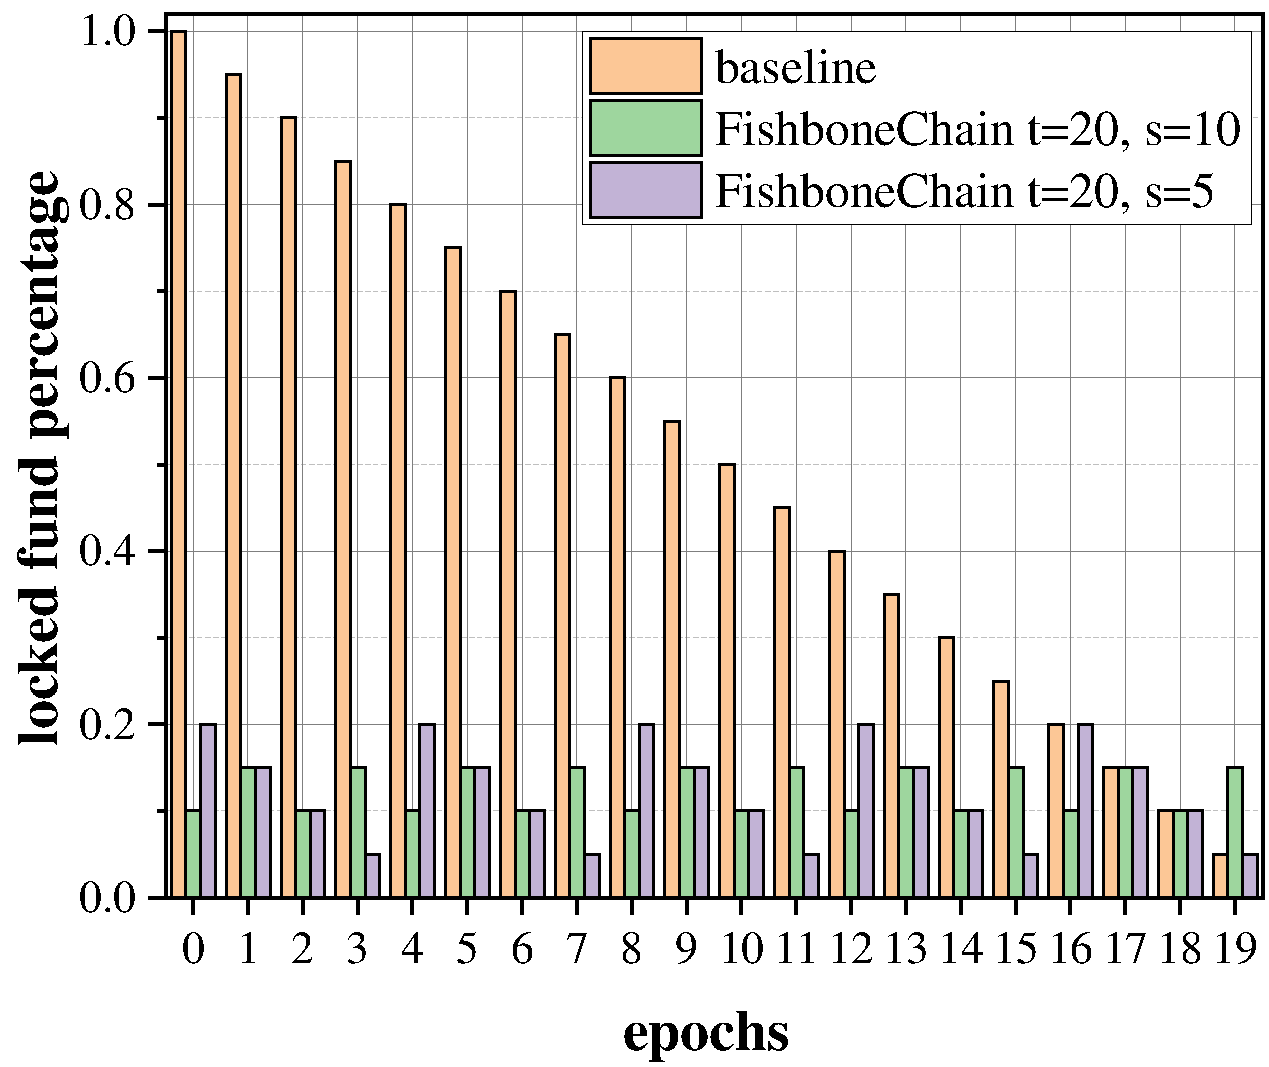
\includegraphics[width=0.55\linewidth]{Round-2/response/figures/locked_fund_comparison.pdf}
    \caption{Comparison of the percentage of locked funds}
    \label{fig:locked_fund_per}
\end{figure}


Next, we analyze the advantages of periodic fund management over the traditional approach. In the baseline scheme, requesters are required to lock individual budgets at the beginning of the task, leading to a potentially substantial accumulation of frozen funds. By contrast, our FishboneChain architecture permits requesters to periodically transfer funds to FMC for budget management, mitigating the locked fund issue. To compare locked fund percentages between the two schemes during task execution, we design a simplified periodic fund management mechanism. Assuming there are $s$ child chains with the same duration of epoch and a requester posts a task on each of them. Each task demands $t$ epochs for completion, and the budget per task is $b$. For the baseline, the requester should lock $L=tb$ for every task separately, which is a $s*t*b$ for frozen funds. For the baseline scheme, the requester needs to lock $L = tb$ funds for each task separately, resulting in a total initial locked amount of $L_{total} = s * L = s * t * b$. In the $i$-th period of $t$ periods, where $i \in [0,t)$, the frozen fund for each task is $F^{baseline}_i = (t-i)b$. In other words, at period $i=1$, the budget of each $T_i$ that is actively used is only $b$, while the remaining $F^{baseline}_1 = (t-1)b$, although not yet used, remains locked. At period $i=2$, the frozen fund for each task is $F^{baseline}_2 = (t-2)b$. At the last period ($i=t$), the frozen fund becomes $F^{baseline}_t = (t-t)b=0$, meaning all budgets are used in this period. Therefore, in the $i$-th period, the proportion of frozen funds in the total budget is $\frac{s*F^{baseline}_i}{s*L} = \frac{(t-i)b}{tb} = \frac{t-i}{t}$. Because the base scheme locks funds on the main chain, each is $tb$. For the convenience of analysis, in our scheme, the requester also locks the same fund $L=tb$ to the main chain at one time but periodically locks these funds in $s$ times. Therefore, at the $i$ epoch, $i \in [0,t)$, the total amount of locked funds is $F^{FishboneChain}_i= tb * (1+ \lfloor \frac{1}{t/s} \rfloor) $ and the total amount of used funds is $i * sb$. Therefore, the locked fund percentage in the $i$ epoch is $\frac{F^{FishboneChain}_i}{i * sb}=[t/s * (1+ \lfloor \frac{1}{t/s} \rfloor) - i]/{t}$.

As shown in Fig.~\ref{fig:locked_fund_per}, the percentage of locked funds is shown for the baseline and our scheme, where two sets of parameters are set for our simplified Fishbonechain scenario. The orange bar represents the baseline scheme, where the requester locks all budgeted funds on the blockchain at the beginning of the task. The green bar illustrates the scenario where the requester publishes 10 tasks on child chains, with each task requiring 20 epochs to complete. The purple bar depicts the scenario of 5 tasks posted on child chains, with each task also requiring 20 epochs for completion. The horizontal axis represents the current period, while the vertical axis shows the percentage of locked funds. It is clear that the percentage of locked funds in our scheme is consistently lower than the baseline scheme, which means that the funds are quickly applied to the task budget for the next epoch. Even if we adjust the number of tasks posted by the requester from 10 to 5, the percentage of locked funds is still less than or equal to $20 \%$. For example, in a data annotation project with 10 child chains, 20 epochs per task, and a \$500 budget per epoch, traditional schemes require locking \$100,000 upfront, while our periodic fund management scheme releases funds gradually. At 25\% completion, our approach only reserves \$15,000-\$20,000 compared to \$75,000 in the traditional approach, freeing substantial capital for other operations. Even in this simplified scenario, implementing a periodic fund management scheme significantly reduces requesters' financial burden. In practical applications with varying task quantities and epoch requirements, requesters can develop fine-grained strategies tailored to their specific needs. This reduced liquidity pressure enables requesters to post more tasks with the same amount of funds, collecting information more comprehensively. The resulting increased platform activity attracts more miners and workers, fostering a positive ecosystem cycle for our Fishbonechain platform.
}\\ %end of color


2. Several important figures, such as Fig. 7 and Fig. 8, are not discussed in sufficient depth. For example, Fig. 8 compares locked fund percentages, but its implications for real-world liquidity and capital efficiency are not analyzed.

{\color{blue}
\noindent \underline{\textbf{Reply:}}

Thanks for your valuable suggestions. We acknowledge that our analysis of Fig. 7 and Fig. 8 in the previous paper lack sufficient depth. We provide a more through and detailed discussion in the revised paper, elaborating on the practical implications of these figures within the crowdsourcing text.

\noindent \underline{\textbf{Modification:}}

For \textbf{Fig. 7}, we add
``
Fig.~\ref{fig:max_tps} serves as a crucial reference framework for the architectural design and scalability planning of real-world crowdsourcing platforms. This performance mapping provides platform architects with precise guidance on system configuration requirements. For instance, when a platform's anticipated transaction volume approaches 10,000 transactions per second, our results demonstrate that maintaining a main chain processing capacity of at least 100 tps is essential to ensure operational stability and service quality. This insight is particularly valuable for large-scale crowdsourcing platforms with user bases in the millions, where transaction demands can fluctuate dramatically. The architectural flexibility illustrated in our results enables significant economic advantages through resource optimization. Platform designers can implement a cost-effective scaling strategy by maintaining moderate main chain performance while dynamically adjusting the number of child chains to accommodate changing demands. Furthermore, our architecture provides a progressive scaling pathway suitable for platforms at various growth stages. Emerging crowdsourcing applications can begin with minimal configurations, like lower main chain tps and fewer child chains, and scale incrementally as their user base expands. ''

For \textbf{Fig. 8}, we add
``
For example, in a data annotation project with 10 child chains, 20 epochs per task, and a \$500 budget per epoch, traditional schemes require locking \$100,000 upfront, while our periodic fund management scheme releases funds gradually. At 25\% completion, our approach only reserves \$15,000-\$20,000 compared to \$75,000 in the traditional approach, freeing substantial capital for other operations. Even in this simplified scenario, implementing a periodic fund management scheme significantly reduces requesters' financial burden. In practical applications with varying task quantities and epoch requirements, requesters can develop fine-grained strategies tailored to their specific needs. This reduced liquidity pressure enables requesters to post more tasks with the same amount of funds, collecting information more comprehensively. The resulting increased platform activity attracts more miners and workers, fostering a positive ecosystem cycle for our Fishbonechain platform.''
}\\ %end of color


3. Some writing and terminology can be improved, especially in the abstract, design goals, and security analysis sections.
We encourage the authors to carefully address the reviewers’ comments accordingly.

{\color{blue}
\noindent \underline{\textbf{Reply and Modification:}}

Thank you for careful reading. We thoroughly proofread the whole paper to address the existing grammatical errors and typographical mistakes.
} %end of color

}